
\documentclass[border=8pt, multi, tikz]{standalone} 
\usepackage{import}
\usepackage{caption}
\subimport{./layers/}{init}
\usetikzlibrary{positioning}
\usetikzlibrary{3d} %for including external image 

\def\ConvColor{rgb:yellow,5;red,2.5;white,5}
\def\ConvReluColor{rgb:yellow,5;red,5;white,5}
\def\PoolColor{rgb:red,1;black,0.3}
\def\AntiPoolColor{rgb:blue,2;green,1;black,0.3}
\def\FcColor{rgb:blue,5;red,2.5;white,5}
\def\FcReluColor{rgb:blue,5;red,5;white,4}
\def\SoftmaxColor{rgb:magenta,5;black,7}   
\def\SumColor{rgb:blue,5;green,15}

\newcommand{\copymidarrow}{\tikz \draw[-Stealth,line width=0.8mm,draw={rgb:blue,4;red,1;green,1;black,3}] (-0.3,0) -- ++(0.3,0);}

\begin{document}
\begin{tikzpicture}
\Large\textbf{My title}
\tikzstyle{connection}=[ultra thick,every node/.style={sloped,allow upside down},draw=\edgecolor,opacity=0.7]
\tikzstyle{copyconnection}=[ultra thick,every node/.style={sloped,allow upside down},draw={rgb:blue,4;red,1;green,1;black,3},opacity=0.7]

\pic[shift={(-1,0,0)}] at (0,0,0) 
    {Box={
        name=input_layer,
        caption= ,
        xlabel={{3, }},
        zlabel= ,
        fill=\ConvColor,
        height=128,
        width=0.1,
        depth=128
        }
    };

\node[canvas is zy plane at x=0] (img_input) at (-3,-2,-5.1) {
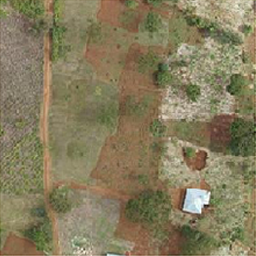
\includegraphics[width=26cm,height=25.8cm]{./images/image1.png},
};
\node[canvas is zy plane at x=0, xscale=-1, inner sep=0pt,above=\abovecaptionskip of img_input,text width=\linewidth]
    {Aerial image shape:(256, 256, 3)};

\pic[shift={(0,0,0)}] at (0,0,0) 
    {Box={
        name=conv0,
        caption=$Encoder (Resnet34) ->$,
        xlabel={{64, }},
        zlabel=128,
        fill=\ConvColor,
        height=64,
        width=4,
        depth=64
        }
    };

\draw [connection]  (input_layer-east)    -- node {\midarrow} (conv0-west);

\pic[shift={ (0,0,0) }] at (conv0-east) 
    {Box={
        name=relu0,
        caption= ,
        fill=\ConvReluColor,
        opacity=0.5,
        height=64,
        width=1,
        depth=64
        }
    };

\pic[shift={ (0,0,0) }] at (relu0-east) 
    {Box={
        name=pooling0,
        caption= ,
        fill=\PoolColor,
        zlabel=64,
        opacity=0.5,
        height=32,
        width=1,
        depth=32
        }
    };

\pic[shift={(3,0,0)}] at (pooling0-east) 
    {Box={
        name=stage1_unit1_conv1,
        caption= ,
        xlabel={{64, }},
        zlabel=64,
        fill=\ConvColor,
        height=32,
        width=4,
        depth=32
        }
    };

\draw [connection]  (pooling0-east)    -- node {\midarrow} (stage1_unit1_conv1-west);

\pic[shift={ (0,0,0) }] at (stage1_unit1_conv1-east) 
    {Box={
        name=stage1_unit1_relu2,
        caption= ,
        fill=\ConvReluColor,
        opacity=0.5,
        height=32,
        width=1,
        depth=32
        }
    };

\pic[shift={(0,0,0)}] at (stage1_unit1_relu2-east) 
    {Box={
        name=stage1_unit1_conv2,
        caption= ,
        xlabel={{64, }},
        zlabel=64,
        fill=\ConvColor,
        height=32,
        width=4,
        depth=32
        }
    };

\pic[shift={(3,10,0)}] at (pooling0-east) 
    {Box={
        name=stage1_unit1_sc,
        caption= ,
        xlabel={{64, }},
        zlabel=64,
        fill=\ConvColor,
        height=32,
        width=4,
        depth=32
        }
    };

\pic[shift={(1,0,0)}] at (stage1_unit1_conv2-east) 
    {Box={
        name=stage1_unit2_conv1,
        caption= ,
        xlabel={{64, }},
        zlabel=64,
        fill=\ConvColor,
        height=32,
        width=4,
        depth=32
        }
    };

\draw [connection]  (stage1_unit1_conv2-east)    -- node {\midarrow} (stage1_unit2_conv1-west);

\path (pooling0-east) -- (stage1_unit1_conv1-west) coordinate[pos=0.4] (after1);
\path (stage1_unit1_conv2-east) -- (stage1_unit2_conv1-west) coordinate[pos=0.4] (before1);
\draw [connection]  (after1)  -- node {\midarrow} ++(0,10,0) -- node {\midarrow} (stage1_unit1_sc-west);
\draw [connection]  (stage1_unit1_sc-east)  -- node {\midarrow} ++(1.4,0,0) -- node {\midarrow} (before1);

\pic[shift={ (0,0,0) }] at (stage1_unit2_conv1-east) 
    {Box={
        name=stage1_unit2_relu2,
        caption= ,
        fill=\ConvReluColor,
        opacity=0.5,
        height=32,
        width=1,
        depth=32
        }
    };

\pic[shift={(0,0,0)}] at (stage1_unit2_relu2-east) 
    {Box={
        name=stage1_unit2_conv2,
        caption= ,
        xlabel={{64, }},
        zlabel=64,
        fill=\ConvColor,
        height=32,
        width=4,
        depth=32
        }
    };

\pic[shift={(1,0,0)}] at (stage1_unit2_conv2-east) 
    {Box={
        name=stage1_unit3_conv1,
        caption= ,
        xlabel={{64, }},
        zlabel=64,
        fill=\ConvColor,
        height=32,
        width=4,
        depth=32
        }
    };

\path (stage1_unit2_conv1-south) -- (stage1_unit2_conv1-north) coordinate[pos=1.25] (stage1_unit2_conv1-top) ;
\path (stage1_unit3_conv1-southwest)  -- (stage1_unit3_conv1-northwest)  coordinate[pos=1.25] (stage1_unit3_conv1-top) ;
\draw [connection]  (stage1_unit2_conv1-north)  
-- node {\midarrow}(stage1_unit2_conv1-top)
-- node {\midarrow}(stage1_unit3_conv1-top)
-- node {\midarrow} (stage1_unit3_conv1-northwest);

\draw [connection]  (stage1_unit2_conv2-east)    -- node {\midarrow} (stage1_unit3_conv1-west);

\pic[shift={ (0,0,0) }] at (stage1_unit3_conv1-east) 
    {Box={
        name=stage1_unit3_relu2,
        caption= ,
        fill=\ConvReluColor,
        opacity=0.5,
        height=32,
        width=1,
        depth=32
        }
    };

\pic[shift={(0,0,0)}] at (stage1_unit3_relu2-east) 
    {Box={
        name=stage1_unit3_conv2,
        caption= ,
        xlabel={{64, }},
        zlabel=64,
        fill=\ConvColor,
        height=32,
        width=4,
        depth=32
        }
    };

\path (stage1_unit3_conv1-south) -- (stage1_unit3_conv1-north) coordinate[pos=1.25] (stage1_unit3_conv1-top) ;
\path (stage1_unit3_conv2-southeast)  -- (stage1_unit3_conv2-northeast)  coordinate[pos=1.25] (stage1_unit3_conv2-top) ;
\draw [connection]  (stage1_unit3_conv1-north)  
-- node {\midarrow}(stage1_unit3_conv1-top)
-- node {\midarrow}(stage1_unit3_conv2-top)
-- node {\midarrow} (stage1_unit3_conv2-northeast);

\pic[shift={(3,0,0)}] at (stage1_unit3_conv2-east) 
    {Box={
        name=stage2_unit1_conv1,
        caption= ,
        xlabel={{128, }},
        zlabel=32,
        fill=\ConvColor,
        height=16,
        width=4,
        depth=16
        }
    };

\draw [connection]  (stage1_unit3_conv2-east)    -- node {\midarrow} (stage2_unit1_conv1-west);

\pic[shift={ (0,0,0) }] at (stage2_unit1_conv1-east) 
    {Box={
        name=stage2_unit1_relu2,
        caption= ,
        fill=\ConvReluColor,
        opacity=0.5,
        height=16,
        width=1,
        depth=16
        }
    };

\pic[shift={(0,0,0)}] at (stage2_unit1_relu2-east) 
    {Box={
        name=stage2_unit1_conv2,
        caption= ,
        xlabel={{128, }},
        zlabel=32,
        fill=\ConvColor,
        height=16,
        width=4,
        depth=16
        }
    };

\pic[shift={(3,5,0)}] at (stage1_unit3_conv2-east) 
    {Box={
        name=stage2_unit1_sc,
        caption= ,
        xlabel={{128, }},
        zlabel=32,
        fill=\ConvColor,
        height=16,
        width=4,
        depth=16
        }
    };

\pic[shift={(1,0,0)}] at (stage2_unit1_conv2-east) 
    {Box={
        name=stage2_unit2_conv1,
        caption= ,
        xlabel={{128, }},
        zlabel=32,
        fill=\ConvColor,
        height=16,
        width=4,
        depth=16
        }
    };

\draw [connection]  (stage2_unit1_conv2-east)    -- node {\midarrow} (stage2_unit2_conv1-west);

\path (stage1_unit3_conv2-east) -- (stage2_unit1_conv1-west) coordinate[pos=0.4] (after1);
\path (stage2_unit1_conv2-east) -- (stage2_unit2_conv1-west) coordinate[pos=0.4] (before1);
\draw [connection]  (after1)  -- node {\midarrow} ++(0,5,0) -- node {\midarrow} (stage2_unit1_sc-west);
\draw [connection]  (stage2_unit1_sc-east)  -- node {\midarrow} ++(1.4,0,0) -- node {\midarrow} (before1);

\pic[shift={ (0,0,0) }] at (stage2_unit2_conv1-east) 
    {Box={
        name=stage2_unit2_relu2,
        caption= ,
        fill=\ConvReluColor,
        opacity=0.5,
        height=16,
        width=1,
        depth=16
        }
    };

\pic[shift={(0,0,0)}] at (stage2_unit2_relu2-east) 
    {Box={
        name=stage2_unit2_conv2,
        caption= ,
        xlabel={{128, }},
        zlabel=32,
        fill=\ConvColor,
        height=16,
        width=4,
        depth=16
        }
    };

\pic[shift={(1,0,0)}] at (stage2_unit2_conv2-east) 
    {Box={
        name=stage2_unit3_conv1,
        caption= ,
        xlabel={{128, }},
        zlabel=32,
        fill=\ConvColor,
        height=16,
        width=4,
        depth=16
        }
    };

\draw [connection]  (stage2_unit2_conv2-east)    -- node {\midarrow} (stage2_unit3_conv1-west);

\path (stage2_unit2_conv1-south) -- (stage2_unit2_conv1-north) coordinate[pos=1.25] (stage2_unit2_conv1-top) ;
\path (stage2_unit3_conv1-southwest)  -- (stage2_unit3_conv1-northwest)  coordinate[pos=1.25] (stage2_unit3_conv1-top) ;
\draw [connection]  (stage2_unit2_conv1-north)  
-- node {\midarrow}(stage2_unit2_conv1-top)
-- node {\midarrow}(stage2_unit3_conv1-top)
-- node {\midarrow} (stage2_unit3_conv1-northwest);

\pic[shift={ (0,0,0) }] at (stage2_unit3_conv1-east) 
    {Box={
        name=stage2_unit3_relu2,
        caption= ,
        fill=\ConvReluColor,
        opacity=0.5,
        height=16,
        width=1,
        depth=16
        }
    };

\pic[shift={(0,0,0)}] at (stage2_unit3_relu2-east) 
    {Box={
        name=stage2_unit3_conv2,
        caption= ,
        xlabel={{128, }},
        zlabel=32,
        fill=\ConvColor,
        height=16,
        width=4,
        depth=16
        }
    };

\pic[shift={(1,0,0)}] at (stage2_unit3_conv2-east) 
    {Box={
        name=stage2_unit4_conv1,
        caption= ,
        xlabel={{128, }},
        zlabel=32,
        fill=\ConvColor,
        height=16,
        width=4,
        depth=16
        }
    };

\draw [connection]  (stage2_unit3_conv2-east)    -- node {\midarrow} (stage2_unit4_conv1-west);

\path (stage2_unit3_conv1-south) -- (stage2_unit3_conv1-north) coordinate[pos=1.25] (stage2_unit3_conv1-top) ;
\path (stage2_unit4_conv1-southwest)  -- (stage2_unit4_conv1-northwest)  coordinate[pos=1.25] (stage2_unit4_conv1-top) ;
\draw [connection]  (stage2_unit3_conv1-north)  
-- node {\midarrow}(stage2_unit3_conv1-top)
-- node {\midarrow}(stage2_unit4_conv1-top)
-- node {\midarrow} (stage2_unit4_conv1-northwest);

\pic[shift={ (0,0,0) }] at (stage2_unit4_conv1-east) 
    {Box={
        name=stage2_unit4_relu2,
        caption= ,
        fill=\ConvReluColor,
        opacity=0.5,
        height=16,
        width=1,
        depth=16
        }
    };

\pic[shift={(0,0,0)}] at (stage2_unit4_relu2-east) 
    {Box={
        name=stage2_unit4_conv2,
        caption= ,
        xlabel={{128, }},
        zlabel=32,
        fill=\ConvColor,
        height=16,
        width=4,
        depth=16
        }
    };

\path (stage2_unit4_conv1-south) -- (stage2_unit4_conv1-north) coordinate[pos=1.25] (stage2_unit4_conv1-top) ;
\path (stage2_unit4_conv2-southeast)  -- (stage2_unit4_conv2-northeast)  coordinate[pos=1.25] (stage2_unit4_conv2-top) ;
\draw [connection]  (stage2_unit4_conv1-north)  
-- node {\midarrow}(stage2_unit4_conv1-top)
-- node {\midarrow}(stage2_unit4_conv2-top)
-- node {\midarrow} (stage2_unit4_conv2-northeast);

\pic[shift={(2,0,0)}] at (stage2_unit4_conv2-east) 
    {Box={
        name=stage3_unit1_conv1,
        caption= ,
        xlabel={{256, }},
        zlabel=16,
        fill=\ConvColor,
        height=8,
        width=4,
        depth=8
        }
    };

\draw [connection]  (stage2_unit4_conv2-east)    -- node {\midarrow} (stage3_unit1_conv1-west);

\pic[shift={ (0,0,0) }] at (stage3_unit1_conv1-east) 
    {Box={
        name=stage3_unit1_relu2,
        caption= ,
        fill=\ConvReluColor,
        opacity=0.5,
        height=8,
        width=1,
        depth=8
        }
    };

\pic[shift={(0,0,0)}] at (stage3_unit1_relu2-east) 
    {Box={
        name=stage3_unit1_conv2,
        caption= ,
        xlabel={{256, }},
        zlabel=16,
        fill=\ConvColor,
        height=8,
        width=4,
        depth=8
        }
    };

\pic[shift={(2,2.5,0)}] at (stage2_unit4_conv2-east) 
    {Box={
        name=stage3_unit1_sc,
        caption= ,
        xlabel={{256, }},
        zlabel=16,
        fill=\ConvColor,
        height=8,
        width=4,
        depth=8
        }
    };

\pic[shift={(1,0,0)}] at (stage3_unit1_conv2-east) 
    {Box={
        name=stage3_unit2_conv1,
        caption= ,
        xlabel={{256, }},
        zlabel=16,
        fill=\ConvColor,
        height=8,
        width=4,
        depth=8
        }
    };

\draw [connection]  (stage3_unit1_conv2-east)    -- node {\midarrow} (stage3_unit2_conv1-west);

\path (stage2_unit4_conv1-east) -- (stage3_unit1_conv1-west) coordinate[pos=0.6] (after1);
\path (stage3_unit1_conv2-east) -- (stage3_unit2_conv1-west) coordinate[pos=0.4] (before1);
\draw [connection]  (after1)  -- node {\midarrow} ++(0,2.5,0) -- node {\midarrow} (stage3_unit1_sc-west);
\draw [connection]  (stage3_unit1_sc-east)  -- node {\midarrow} ++(1.4,0,0) -- node {\midarrow} (before1);

\pic[shift={ (0,0,0) }] at (stage3_unit2_conv1-east) 
    {Box={
        name=stage3_unit2_relu2,
        caption= ,
        fill=\ConvReluColor,
        opacity=0.5,
        height=8,
        width=1,
        depth=8
        }
    };

\pic[shift={(0,0,0)}] at (stage3_unit2_relu2-east) 
    {Box={
        name=stage3_unit2_conv2,
        caption= ,
        xlabel={{256, }},
        zlabel=16,
        fill=\ConvColor,
        height=8,
        width=4,
        depth=8
        }
    };

\pic[shift={(1,0,0)}] at (stage3_unit2_conv2-east) 
    {Box={
        name=stage3_unit3_conv1,
        caption= ,
        xlabel={{256, }},
        zlabel=16,
        fill=\ConvColor,
        height=8,
        width=4,
        depth=8
        }
    };

\draw [connection]  (stage3_unit2_conv2-east)    -- node {\midarrow} (stage3_unit3_conv1-west);

\path (stage3_unit2_conv1-south) -- (stage3_unit2_conv1-north) coordinate[pos=1.5] (stage3_unit2_conv1-top) ;
\path (stage3_unit3_conv1-southwest)  -- (stage3_unit3_conv1-northwest)  coordinate[pos=1.5] (stage3_unit3_conv1-top) ;
\draw [connection]  (stage3_unit2_conv1-north)  
-- node {\midarrow}(stage3_unit2_conv1-top)
-- node {\midarrow}(stage3_unit3_conv1-top)
-- node {\midarrow} (stage3_unit3_conv1-northwest);

\pic[shift={ (0,0,0) }] at (stage3_unit3_conv1-east) 
    {Box={
        name=stage3_unit3_relu2,
        caption= ,
        fill=\ConvReluColor,
        opacity=0.5,
        height=8,
        width=1,
        depth=8
        }
    };

\pic[shift={(0,0,0)}] at (stage3_unit3_relu2-east) 
    {Box={
        name=stage3_unit3_conv2,
        caption= ,
        xlabel={{256, }},
        zlabel=16,
        fill=\ConvColor,
        height=8,
        width=4,
        depth=8
        }
    };

\pic[shift={(1,0,0)}] at (stage3_unit3_conv2-east) 
    {Box={
        name=stage3_unit4_conv1,
        caption= ,
        xlabel={{256, }},
        zlabel=16,
        fill=\ConvColor,
        height=8,
        width=4,
        depth=8
        }
    };

\draw [connection]  (stage3_unit3_conv2-east)    -- node {\midarrow} (stage3_unit4_conv1-west);

\path (stage3_unit3_conv1-south) -- (stage3_unit3_conv1-north) coordinate[pos=1.5] (stage3_unit3_conv1-top) ;
\path (stage3_unit4_conv1-southwest)  -- (stage3_unit4_conv1-northwest)  coordinate[pos=1.5] (stage3_unit4_conv1-top) ;
\draw [connection]  (stage3_unit3_conv1-north)  
-- node {\midarrow}(stage3_unit3_conv1-top)
-- node {\midarrow}(stage3_unit4_conv1-top)
-- node {\midarrow} (stage3_unit4_conv1-northwest);

\pic[shift={ (0,0,0) }] at (stage3_unit4_conv1-east) 
    {Box={
        name=stage3_unit4_relu2,
        caption= ,
        fill=\ConvReluColor,
        opacity=0.5,
        height=8,
        width=1,
        depth=8
        }
    };

\pic[shift={(0,0,0)}] at (stage3_unit4_relu2-east) 
    {Box={
        name=stage3_unit4_conv2,
        caption= ,
        xlabel={{256, }},
        zlabel=16,
        fill=\ConvColor,
        height=8,
        width=4,
        depth=8
        }
    };

\pic[shift={(1,0,0)}] at (stage3_unit4_conv2-east) 
    {Box={
        name=stage3_unit5_conv1,
        caption= ,
        xlabel={{256, }},
        zlabel=16,
        fill=\ConvColor,
        height=8,
        width=4,
        depth=8
        }
    };

\draw [connection]  (stage3_unit4_conv2-east)    -- node {\midarrow} (stage3_unit5_conv1-west);

\path (stage3_unit4_conv1-south) -- (stage3_unit4_conv1-north) coordinate[pos=1.5] (stage3_unit4_conv1-top) ;
\path (stage3_unit5_conv1-southwest)  -- (stage3_unit5_conv1-northwest)  coordinate[pos=1.5] (stage3_unit5_conv1-top) ;
\draw [connection]  (stage3_unit4_conv1-north)  
-- node {\midarrow}(stage3_unit4_conv1-top)
-- node {\midarrow}(stage3_unit5_conv1-top)
-- node {\midarrow} (stage3_unit5_conv1-northwest);

\pic[shift={ (0,0,0) }] at (stage3_unit5_conv1-east) 
    {Box={
        name=stage3_unit5_relu2,
        caption= ,
        fill=\ConvReluColor,
        opacity=0.5,
        height=8,
        width=1,
        depth=8
        }
    };

\pic[shift={(0,0,0)}] at (stage3_unit5_relu2-east) 
    {Box={
        name=stage3_unit5_conv2,
        caption= ,
        xlabel={{256, }},
        zlabel=16,
        fill=\ConvColor,
        height=8,
        width=4,
        depth=8
        }
    };

\pic[shift={(1,0,0)}] at (stage3_unit5_conv2-east) 
    {Box={
        name=stage3_unit6_conv1,
        caption= ,
        xlabel={{256, }},
        zlabel=16,
        fill=\ConvColor,
        height=8,
        width=4,
        depth=8
        }
    };

\draw [connection]  (stage3_unit5_conv2-east)    -- node {\midarrow} (stage3_unit6_conv1-west);

\path (stage3_unit5_conv1-south) -- (stage3_unit5_conv1-north) coordinate[pos=1.5] (stage3_unit5_conv1-top) ;
\path (stage3_unit6_conv1-southwest)  -- (stage3_unit6_conv1-northwest)  coordinate[pos=1.5] (stage3_unit6_conv1-top) ;
\draw [connection]  (stage3_unit5_conv1-north)  
-- node {\midarrow}(stage3_unit5_conv1-top)
-- node {\midarrow}(stage3_unit6_conv1-top)
-- node {\midarrow} (stage3_unit6_conv1-northwest);

\pic[shift={ (0,0,0) }] at (stage3_unit6_conv1-east) 
    {Box={
        name=stage3_unit6_relu2,
        caption= ,
        fill=\ConvReluColor,
        opacity=0.5,
        height=8,
        width=1,
        depth=8
        }
    };

\pic[shift={(0,0,0)}] at (stage3_unit6_relu2-east) 
    {Box={
        name=stage3_unit6_conv2,
        caption= ,
        xlabel={{256, }},
        zlabel=16,
        fill=\ConvColor,
        height=8,
        width=4,
        depth=8
        }
    };

\path (stage3_unit6_conv1-south) -- (stage3_unit6_conv1-north) coordinate[pos=1.5] (stage3_unit6_conv1-top) ;
\path (stage3_unit6_conv2-southeast)  -- (stage3_unit6_conv2-northeast)  coordinate[pos=1.5] (stage3_unit6_conv2-top) ;
\draw [connection]  (stage3_unit6_conv1-north)  
-- node {\midarrow}(stage3_unit6_conv1-top)
-- node {\midarrow}(stage3_unit6_conv2-top)
-- node {\midarrow} (stage3_unit6_conv2-northeast);

\pic[shift={(1.5,0,0)}] at (stage3_unit6_conv2-east) 
    {Box={
        name=stage4_unit1_conv1,
        caption= ,
        xlabel={{512, }},
        zlabel=8,
        fill=\ConvColor,
        height=4,
        width=4,
        depth=4
        }
    };

\draw [connection]  (stage2_unit4_conv2-east)    -- node {\midarrow} (stage4_unit1_conv1-west);

\pic[shift={ (0,0,0) }] at (stage4_unit1_conv1-east) 
    {Box={
        name=stage4_unit1_relu2,
        caption= ,
        fill=\ConvReluColor,
        opacity=0.5,
        height=4,
        width=1,
        depth=4
        }
    };

\pic[shift={(0,0,0)}] at (stage4_unit1_relu2-east) 
    {Box={
        name=stage4_unit1_conv2,
        caption= ,
        xlabel={{512, }},
        zlabel=8,
        fill=\ConvColor,
        height=4,
        width=4,
        depth=4
        }
    };

\pic[shift={(1.5,2.5,0)}] at (stage3_unit6_conv2-east) 
    {Box={
        name=stage4_unit1_sc,
        caption= ,
        xlabel={{512, }},
        zlabel=8,
        fill=\ConvColor,
        height=4,
        width=4,
        depth=4
        }
    };

\pic[shift={(1,0,0)}] at (stage4_unit1_conv2-east) 
    {Box={
        name=stage4_unit2_conv1,
        caption= ,
        xlabel={{512, }},
        zlabel=8,
        fill=\ConvColor,
        height=4,
        width=4,
        depth=4
        }
    };

\draw [connection]  (stage4_unit1_conv2-east)    -- node {\midarrow} (stage4_unit2_conv1-west);

\path (stage3_unit6_conv1-east) -- (stage4_unit1_conv1-west) coordinate[pos=0.6] (after1);
\path (stage4_unit1_conv2-east) -- (stage4_unit2_conv1-west) coordinate[pos=0.4] (before1);
\draw [connection]  (after1)  -- node {\midarrow} ++(0,2.5,0) -- node {\midarrow} (stage4_unit1_sc-west);
\draw [connection]  (stage4_unit1_sc-east)  -- node {\midarrow} ++(1.4,0,0) -- node {\midarrow} (before1);

\pic[shift={ (0,0,0) }] at (stage4_unit2_conv1-east) 
    {Box={
        name=stage4_unit2_relu2,
        caption= ,
        fill=\ConvReluColor,
        opacity=0.5,
        height=4,
        width=1,
        depth=4
        }
    };

\pic[shift={(0,0,0)}] at (stage4_unit2_relu2-east) 
    {Box={
        name=stage4_unit2_conv2,
        caption= ,
        xlabel={{512, }},
        zlabel=8,
        fill=\ConvColor,
        height=4,
        width=4,
        depth=4
        }
    };

\pic[shift={(1,0,0)}] at (stage4_unit2_conv2-east) 
    {Box={
        name=stage4_unit3_conv1,
        caption= ,
        xlabel={{512, }},
        zlabel=8,
        fill=\ConvColor,
        height=4,
        width=4,
        depth=4
        }
    };

\draw [connection]  (stage4_unit2_conv2-east)    -- node {\midarrow} (stage4_unit3_conv1-west);

\path (stage4_unit2_conv1-south) -- (stage4_unit2_conv1-north) coordinate[pos=1.7] (stage4_unit2_conv1-top) ;
\path (stage4_unit3_conv1-southwest)  -- (stage4_unit3_conv1-northwest)  coordinate[pos=1.75] (stage4_unit3_conv1-top) ;
\draw [connection]  (stage4_unit2_conv1-north)  
-- node {\midarrow}(stage4_unit2_conv1-top)
-- node {\midarrow}(stage4_unit3_conv1-top)
-- node {\midarrow} (stage4_unit3_conv1-northwest);

\pic[shift={ (0,0,0) }] at (stage4_unit3_conv1-east) 
    {Box={
        name=stage4_unit3_relu2,
        caption= ,
        fill=\ConvReluColor,
        opacity=0.5,
        height=4,
        width=1,
        depth=4
        }
    };

\pic[shift={(0,0,0)}] at (stage4_unit3_relu2-east) 
    {Box={
        name=stage4_unit3_conv2,
        caption=$Bottleneck ->$,
        xlabel={{512, }},
        zlabel=8,
        fill=\ConvColor,
        height=4,
        width=4,
        depth=4
        }
    };

\path (stage4_unit3_conv1-south) -- (stage4_unit3_conv1-north) coordinate[pos=1.75] (stage4_unit3_conv1-top) ;
\path (stage4_unit3_conv2-southeast)  -- (stage4_unit3_conv2-northeast)  coordinate[pos=1.75] (stage4_unit3_conv2-top) ;
\draw [connection]  (stage4_unit3_conv1-north)  
-- node {\midarrow}(stage4_unit3_conv1-top)
-- node {\midarrow}(stage4_unit3_conv2-top)
-- node {\midarrow} (stage4_unit3_conv2-northeast);

\pic[shift={ (2,0,0) }] at (stage4_unit3_conv1-east) 
    {Box={
        name=block4_mxp,
        caption= ,
        fill=\PoolColor,
        zlabel=4,
        opacity=0.5,
        height=2,
        width=1,
        depth=2
        }
    };

\draw [connection]  (stage4_unit3_conv2-east)    -- node {\midarrow} (block4_mxp-west);

\pic[shift={(0,0,0)}] at (block4_mxp-east) 
    {Box={
        name=btn_conv1,
        caption= ,
        xlabel={{256, }},
        zlabel=4,
        fill=\ConvColor,
        height=2,
        width=4,
        depth=2
        }
    };

\pic[shift={(0,0,0)}] at (block4_mxp-east) 
    {Box={
        name=btn_conv2,
        caption= ,
        xlabel={{256, }},
        zlabel=4,
        fill=\ConvColor,
        height=2,
        width=4,
        depth=2
        }
    };

\path (block4_mxp-south) -- (block4_mxp-north) coordinate[pos=2.5] (block4_mxp-top) ;
\path (btn_conv2-southeast)  -- (btn_conv2-northeast)  coordinate[pos=2.5] (btn_conv2-top) ;
\draw [connection]  (block4_mxp-north)  
-- node {\midarrow}(block4_mxp-top)
-- node {\midarrow}(btn_conv2-top)
-- node {\midarrow} (btn_conv2-northeast);

\path (stage4_unit3_conv2-southeast) -- (stage4_unit3_conv2-northeast) coordinate[pos=2] (stage4_unit3_conv2-top) ;
\path (block4_mxp-southwest)  -- (block4_mxp-northwest)  coordinate[pos=3.5] (block4_mxp-top) ;
\draw [connection]  (stage4_unit3_conv2-northeast)  
-- node {\midarrow}(stage4_unit3_conv2-top)
-- node {\midarrow}(block4_mxp-top)
-- node {\midarrow} (block4_mxp-northwest);

\pic[shift={(0,0,0)}] at (btn_conv2-east) 
    {Box={
        name=btn_upconv1,
        caption= ,
        xlabel={{128, }},
        zlabel=8,
        fill=\AntiPoolColor,
        height=4,
        width=4,
        depth=4
        }
    };

\draw [connection]  (btn_conv2-east)    -- node {\midarrow} (btn_upconv1-west);

\path (block4_mxp-southwest) -- (block4_mxp-northwest) coordinate[pos=4] (block4_mxp-top) ;
\path (btn_upconv1-southeast)  -- (btn_upconv1-northeast)  coordinate[pos=2.25] (btn_upconv1-top) ;
\draw [connection]  (block4_mxp-northwest)  
-- node {\midarrow}(block4_mxp-top)
-- node {\midarrow}(btn_upconv1-top)
-- node {\midarrow} (btn_upconv1-northeast);

\pic[shift={(1,0,0)}] at (btn_upconv1-east) 
    {Box={
        name=de_block1_conv0,
        caption=$Decoder ->$,
        xlabel={{256, }},
        zlabel=8,
        fill=\ConvColor,
        height=4,
        width=4,
        depth=4
        }
    };

\draw [connection]  (btn_upconv1-east)    -- node {\midarrow} (de_block1_conv0-west);

\pic[shift={ (0,0,0) }] at (de_block1_conv0-east) 
    {Box={
        name=de_block1_relu0,
        caption= ,
        fill=\ConvReluColor,
        opacity=0.5,
        height=4,
        width=1,
        depth=4
        }
    };

\pic[shift={(0,0,0)}] at (de_block1_relu0-east) 
    {Box={
        name=de_block1_conv1,
        caption= ,
        xlabel={{128, }},
        zlabel=8,
        fill=\ConvColor,
        height=4,
        width=4,
        depth=4
        }
    };

\pic[shift={ (0,0,0) }] at (de_block1_conv1-east) 
    {Box={
        name=de_block1_relu1,
        caption= ,
        fill=\ConvReluColor,
        opacity=0.5,
        height=4,
        width=1,
        depth=4
        }
    };

\pic[shift={(0,0,0)}] at (de_block1_relu1-east) 
    {Box={
        name=de_block1_conv2,
        caption= ,
        xlabel={{256, }},
        zlabel=8,
        fill=\ConvColor,
        height=4,
        width=4,
        depth=4
        }
    };

\pic[shift={ (0,0,0) }] at (de_block1_conv2-east) 
    {Box={
        name=de_block1_relu2,
        caption= ,
        fill=\ConvReluColor,
        opacity=0.5,
        height=4,
        width=1,
        depth=4
        }
    };

\pic[shift={(1,0,0)}] at (de_block1_relu2-east) 
    {Box={
        name=de_block1_upconv1,
        caption= ,
        xlabel={{256, }},
        zlabel=16,
        fill=\AntiPoolColor,
        height=8,
        width=4,
        depth=8
        }
    };

\draw [connection]  (de_block1_relu2-east)    -- node {\midarrow} (de_block1_upconv1-west);

\path (btn_upconv1-southeast) -- (btn_upconv1-northeast) coordinate[pos=3] (btn_upconv1-top) ;
\path (de_block1_upconv1-southwest)  -- (de_block1_upconv1-northwest)  coordinate[pos=1.75] (de_block1_upconv1-top) ;
\draw [connection]  (btn_upconv1-northeast)  
-- node {\midarrow}(btn_upconv1-top)
-- node {\midarrow}(de_block1_upconv1-top)
-- node {\midarrow} (de_block1_upconv1-northwest);

\path (stage4_unit1_conv1-northwest) -- (stage4_unit1_conv1-southwest) coordinate[pos=3] (stage4_unit1_conv1-top) ;
\path (de_block1_upconv1-northeast)  -- (de_block1_upconv1-southeast)  coordinate[pos=1.75] (de_block1_upconv1-top) ;
\draw [connection]  (stage4_unit1_conv1-southwest)  
-- node {\midarrow}(stage4_unit1_conv1-top)
-- node {\midarrow}(de_block1_upconv1-top)
-- node {\midarrow} (de_block1_upconv1-southeast);

\pic[shift={(1,0,0)}] at (de_block1_upconv1-east) 
    {Box={
        name=de_block2_conv0,
        caption= ,
        xlabel={{128, }},
        zlabel=16,
        fill=\ConvColor,
        height=8,
        width=4,
        depth=8
        }
    };

\draw [connection]  (de_block1_upconv1-east)    -- node {\midarrow} (de_block2_conv0-west);

\pic[shift={ (0,0,0) }] at (de_block2_conv0-east) 
    {Box={
        name=de_block2_relu0,
        caption= ,
        fill=\ConvReluColor,
        opacity=0.5,
        height=8,
        width=1,
        depth=8
        }
    };

\pic[shift={(0,0,0)}] at (de_block2_relu0-east) 
    {Box={
        name=de_block2_conv1,
        caption= ,
        xlabel={{64, }},
        zlabel=16,
        fill=\ConvColor,
        height=8,
        width=4,
        depth=8
        }
    };

\pic[shift={ (0,0,0) }] at (de_block2_conv1-east) 
    {Box={
        name=de_block2_relu1,
        caption= ,
        fill=\ConvReluColor,
        opacity=0.5,
        height=8,
        width=1,
        depth=8
        }
    };

\pic[shift={(0,0,0)}] at (de_block2_relu1-east) 
    {Box={
        name=de_block2_conv2,
        caption= ,
        xlabel={{128, }},
        zlabel=16,
        fill=\ConvColor,
        height=8,
        width=4,
        depth=8
        }
    };

\pic[shift={ (0,0,0) }] at (de_block2_conv2-east) 
    {Box={
        name=de_block2_relu2,
        caption= ,
        fill=\ConvReluColor,
        opacity=0.5,
        height=8,
        width=1,
        depth=8
        }
    };

\pic[shift={(1,0,0)}] at (de_block2_relu2-east) 
    {Box={
        name=de_block2_upconv1,
        caption= ,
        xlabel={{128, }},
        zlabel=32,
        fill=\AntiPoolColor,
        height=16,
        width=4,
        depth=16
        }
    };

\draw [connection]  (de_block2_relu2-east)    -- node {\midarrow} (de_block2_upconv1-west);

\path (de_block1_upconv1-southeast) -- (de_block1_upconv1-northeast) coordinate[pos=2.5] (de_block1_upconv1-top) ;
\path (de_block2_upconv1-southwest)  -- (de_block2_upconv1-northwest)  coordinate[pos=1.5] (de_block2_upconv1-top) ;
\draw [connection]  (de_block1_upconv1-northeast)  
-- node {\midarrow}(de_block1_upconv1-top)
-- node {\midarrow}(de_block2_upconv1-top)
-- node {\midarrow} (de_block2_upconv1-northwest);

\path (stage2_unit4_conv2-northwest) -- (stage2_unit4_conv2-southwest) coordinate[pos=1.75] (stage2_unit4_conv2-top) ;
\path (de_block2_upconv1-northeast)  -- (de_block2_upconv1-southeast)  coordinate[pos=1.75] (de_block2_upconv1-top) ;
\draw [connection]  (stage2_unit4_conv2-southwest)  
-- node {\midarrow}(stage2_unit4_conv2-top)
-- node {\midarrow}(de_block2_upconv1-top)
-- node {\midarrow} (de_block2_upconv1-southeast);

\pic[shift={(1,0,0)}] at (de_block2_upconv1-east) 
    {Box={
        name=de_block3_conv0,
        caption= ,
        xlabel={{64, }},
        zlabel=32,
        fill=\ConvColor,
        height=16,
        width=4,
        depth=16
        }
    };

\draw [connection]  (de_block2_upconv1-east)    -- node {\midarrow} (de_block3_conv0-west);

\pic[shift={ (0,0,0) }] at (de_block3_conv0-east) 
    {Box={
        name=de_block3_relu0,
        caption= ,
        fill=\ConvReluColor,
        opacity=0.5,
        height=16,
        width=1,
        depth=16
        }
    };

\pic[shift={(0,0,0)}] at (de_block3_relu0-east) 
    {Box={
        name=de_block3_conv1,
        caption= ,
        xlabel={{32, }},
        zlabel=32,
        fill=\ConvColor,
        height=16,
        width=4,
        depth=16
        }
    };

\pic[shift={ (0,0,0) }] at (de_block3_conv1-east) 
    {Box={
        name=de_block3_relu1,
        caption= ,
        fill=\ConvReluColor,
        opacity=0.5,
        height=16,
        width=1,
        depth=16
        }
    };

\pic[shift={(0,0,0)}] at (de_block3_relu1-east) 
    {Box={
        name=de_block3_conv2,
        caption= ,
        xlabel={{64, }},
        zlabel=32,
        fill=\ConvColor,
        height=16,
        width=4,
        depth=16
        }
    };

\pic[shift={ (0,0,0) }] at (de_block3_conv2-east) 
    {Box={
        name=de_block3_relu2,
        caption= ,
        fill=\ConvReluColor,
        opacity=0.5,
        height=16,
        width=1,
        depth=16
        }
    };

\pic[shift={(1,0,0)}] at (de_block3_relu2-east) 
    {Box={
        name=de_block3_upconv1,
        caption= ,
        xlabel={{64, }},
        zlabel=64,
        fill=\AntiPoolColor,
        height=32,
        width=4,
        depth=32
        }
    };

\draw [connection]  (de_block3_relu2-east)    -- node {\midarrow} (de_block3_upconv1-west);

\path (stage1_unit3_conv2-northwest) -- (stage1_unit3_conv2-southwest) coordinate[pos=1.75] (stage1_unit3_conv2-top) ;
\path (de_block3_upconv1-northeast)  -- (de_block3_upconv1-southeast)  coordinate[pos=1.75] (de_block3_upconv1-top) ;
\draw [connection]  (stage1_unit3_conv2-southwest)  
-- node {\midarrow}(stage1_unit3_conv2-top)
-- node {\midarrow}(de_block3_upconv1-top)
-- node {\midarrow} (de_block3_upconv1-southeast);

\path (de_block2_upconv1-southeast) -- (de_block2_upconv1-northeast) coordinate[pos=2] (de_block2_upconv1-top) ;
\path (de_block3_upconv1-southwest)  -- (de_block3_upconv1-northwest)  coordinate[pos=1.25] (de_block3_upconv1-top) ;
\draw [connection]  (de_block2_upconv1-northeast)  
-- node {\midarrow}(de_block2_upconv1-top)
-- node {\midarrow}(de_block3_upconv1-top)
-- node {\midarrow} (de_block3_upconv1-northwest);

\pic[shift={(1,0,0)}] at (de_block3_upconv1-east) 
    {Box={
        name=de_block4_conv0,
        caption= ,
        xlabel={{32, }},
        zlabel=64,
        fill=\ConvColor,
        height=32,
        width=4,
        depth=32
        }
    };

\draw [connection]  (de_block3_upconv1-east)    -- node {\midarrow} (de_block4_conv0-west);

\pic[shift={ (0,0,0) }] at (de_block4_conv0-east) 
    {Box={
        name=de_block4_relu0,
        caption= ,
        fill=\ConvReluColor,
        opacity=0.5,
        height=32,
        width=1,
        depth=32
        }
    };

\pic[shift={(0,0,0)}] at (de_block4_relu0-east) 
    {Box={
        name=de_block4_conv1,
        caption= ,
        xlabel={{16, }},
        zlabel=64,
        fill=\ConvColor,
        height=32,
        width=4,
        depth=32
        }
    };

\pic[shift={ (0,0,0) }] at (de_block4_conv1-east) 
    {Box={
        name=de_block4_relu1,
        caption= ,
        fill=\ConvReluColor,
        opacity=0.5,
        height=32,
        width=1,
        depth=32
        }
    };

\pic[shift={(0,0,0)}] at (de_block4_relu1-east) 
    {Box={
        name=de_block4_conv2,
        caption= ,
        xlabel={{32, }},
        zlabel=64,
        fill=\ConvColor,
        height=32,
        width=4,
        depth=32
        }
    };

\pic[shift={ (0,0,0) }] at (de_block4_conv2-east) 
    {Box={
        name=de_block4_relu2,
        caption= ,
        fill=\ConvReluColor,
        opacity=0.5,
        height=32,
        width=1,
        depth=32
        }
    };

\pic[shift={(1,0,0)}] at (de_block4_relu2-east) 
    {Box={
        name=de_block4_upconv1,
        caption= ,
        xlabel={{32, }},
        zlabel=128,
        fill=\AntiPoolColor,
        height=64,
        width=4,
        depth=64
        }
    };

\draw [connection]  (de_block3_relu2-east)    -- node {\midarrow} (de_block4_upconv1-west);

\path (conv0-northwest) -- (conv0-southwest) coordinate[pos=1.25] (conv0-top) ;
\path (de_block4_upconv1-northeast)  -- (de_block4_upconv1-southeast)  coordinate[pos=1.25] (de_block4_upconv1-top) ;
\draw [connection]  (conv0-southwest)  
-- node {\midarrow}(conv0-top)
-- node {\midarrow}(de_block4_upconv1-top)
-- node {\midarrow} (de_block4_upconv1-southeast);

\path (de_block3_upconv1-southeast) -- (de_block3_upconv1-northeast) coordinate[pos=1.75] (de_block3_upconv1-top) ;
\path (de_block4_upconv1-southwest)  -- (de_block4_upconv1-northwest)  coordinate[pos=1.125] (de_block4_upconv1-top) ;
\draw [connection]  (de_block3_upconv1-northeast)  
-- node {\midarrow}(de_block3_upconv1-top)
-- node {\midarrow}(de_block4_upconv1-top)
-- node {\midarrow} (de_block4_upconv1-northwest);

\pic[shift={(1,0,0)}] at (de_block4_upconv1-east) 
    {Box={
        name=de_block5_conv0,
        caption= ,
        xlabel={{32, }},
        zlabel=128,
        fill=\ConvColor,
        height=64,
        width=4,
        depth=64
        }
    };

\draw [connection]  (de_block4_upconv1-east)    -- node {\midarrow} (de_block5_conv0-west);

\pic[shift={ (0,0,0) }] at (de_block5_conv0-east) 
    {Box={
        name=de_block5_relu0,
        caption= ,
        fill=\ConvReluColor,
        opacity=0.5,
        height=64,
        width=1,
        depth=64
        }
    };

\pic[shift={(0,0,0)}] at (de_block5_relu0-east) 
    {Box={
        name=de_block5_conv1,
        caption= ,
        xlabel={{16, }},
        zlabel=128,
        fill=\ConvColor,
        height=64,
        width=4,
        depth=64
        }
    };

\pic[shift={ (0,0,0) }] at (de_block5_conv1-east) 
    {Box={
        name=de_block5_relu1,
        caption= ,
        fill=\ConvReluColor,
        opacity=0.5,
        height=64,
        width=1,
        depth=64
        }
    };

\pic[shift={(0,0,0)}] at (de_block5_relu1-east) 
    {Box={
        name=de_block5_conv2,
        caption= ,
        xlabel={{32, }},
        zlabel=128,
        fill=\ConvColor,
        height=64,
        width=4,
        depth=64
        }
    };

\pic[shift={ (0,0,0) }] at (de_block5_conv2-east) 
    {Box={
        name=de_block5_relu2,
        caption= ,
        fill=\ConvReluColor,
        opacity=0.5,
        height=64,
        width=1,
        depth=64
        }
    };

\pic[shift={(1,0,0)}] at (de_block5_relu2-east) 
    {Box={
        name=de_block5_upconv1,
        caption= ,
        xlabel={{32, }},
        zlabel=256,
        fill=\AntiPoolColor,
        height=128,
        width=4,
        depth=128
        }
    };

\draw [connection]  (de_block4_relu2-east)    -- node {\midarrow} (de_block5_upconv1-west);

\path (input_layer-northwest) -- (input_layer-southwest) coordinate[pos=1.25] (input_layer-top) ;
\path (de_block5_upconv1-northeast)  -- (de_block5_upconv1-southeast)  coordinate[pos=1.25] (de_block5_upconv1-top) ;
\draw [connection]  (input_layer-southwest)  
-- node {\midarrow}(input_layer-top)
-- node {\midarrow}(de_block5_upconv1-top)
-- node {\midarrow} (de_block5_upconv1-southeast);

\path (de_block4_upconv1-southeast) -- (de_block4_upconv1-northeast) coordinate[pos=1.75] (de_block4_upconv1-top) ;
\path (de_block5_upconv1-southwest)  -- (de_block5_upconv1-northwest)  coordinate[pos=1.125] (de_block5_upconv1-top) ;
\draw [connection]  (de_block4_upconv1-northeast)  
-- node {\midarrow}(de_block4_upconv1-top)
-- node {\midarrow}(de_block5_upconv1-top)
-- node {\midarrow} (de_block5_upconv1-northwest);

\pic[shift={(1,0,0)}] at (de_block5_upconv1-east) 
    {Box={
        name=de_block6_conv0,
        caption= ,
        xlabel={{16, }},
        zlabel=256,
        fill=\ConvColor,
        height=128,
        width=4,
        depth=128
        }
    };

\draw [connection]  (de_block5_upconv1-east)    -- node {\midarrow} (de_block6_conv0-west);

\pic[shift={ (0,0,0) }] at (de_block6_conv0-east) 
    {Box={
        name=de_block6_relu0,
        caption= ,
        fill=\ConvReluColor,
        opacity=0.5,
        height=128,
        width=1,
        depth=128
        }
    };

\pic[shift={(0,0,0)}] at (de_block6_relu0-east) 
    {Box={
        name=de_block6_conv1,
        caption= ,
        xlabel={{8, }},
        zlabel=256,
        fill=\ConvColor,
        height=128,
        width=4,
        depth=128
        }
    };

\pic[shift={ (0,0,0) }] at (de_block6_conv1-east) 
    {Box={
        name=de_block6_relu1,
        caption= ,
        fill=\ConvReluColor,
        opacity=0.5,
        height=128,
        width=1,
        depth=128
        }
    };

\pic[shift={(0,0,0)}] at (de_block6_relu1-east) 
    {Box={
        name=de_block6_conv2,
        caption= ,
        xlabel={{16, }},
        zlabel=256,
        fill=\ConvColor,
        height=128,
        width=4,
        depth=128
        }
    };

\pic[shift={ (0,0,0) }] at (de_block6_conv2-east) 
    {Box={
        name=de_block6_relu2,
        caption= ,
        fill=\ConvReluColor,
        opacity=0.5,
        height=128,
        width=1,
        depth=128
        }
    };

\pic[shift={(1,0,0)}] at (de_block6_relu2-east) 
    {Box={
        name=de_block7_conv1,
        caption= ,
        xlabel={{8, }},
        zlabel=256,
        fill=\ConvColor,
        height=128,
        width=4,
        depth=128
        }
    };

\pic[shift={ (0,0,0) }] at (de_block7_conv1-east) 
    {Box={
        name=de_block7_relu0,
        caption= ,
        fill=\ConvReluColor,
        opacity=0.5,
        height=128,
        width=1,
        depth=128
        }
    };

\pic[shift={(0.25,0,0)}] at (de_block7_relu0-east) 
    {Box={
        name=output_layer0,
        caption= ,
        xlabel={{1, }},
        zlabel= ,
        fill=\ConvColor,
        height=128,
        width=0.1,
        depth=128
        }
    };

\node[canvas is zy plane at x=0] (img_output0) at (output_layer0-east) {
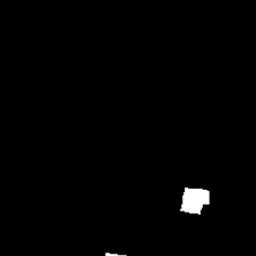
\includegraphics[width=26cm,height=25.8cm]{./images/build1.png},
};
\node[canvas is zy plane at x=0, xscale=-1, inner sep=0pt,above=\abovecaptionskip of img_output0,text width=\linewidth]
    { };

\pic[shift={(0.25,0,0)}] at (output_layer0-east) 
    {Box={
        name=output_layer1,
        caption= ,
        xlabel={{1, }},
        zlabel= ,
        fill=\ConvColor,
        height=128,
        width=0.1,
        depth=128
        }
    };

\node[canvas is zy plane at x=0] (img_output1) at (output_layer1-east) {
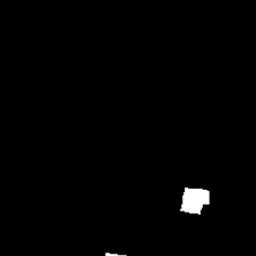
\includegraphics[width=26cm,height=25.8cm]{./images/build1.png},
};
\node[canvas is zy plane at x=0, xscale=-1, inner sep=0pt,above=\abovecaptionskip of img_output1,text width=\linewidth]
    { };

\pic[shift={(0.25,0,0)}] at (output_layer1-east) 
    {Box={
        name=output_layer2,
        caption= ,
        xlabel={{1, }},
        zlabel= ,
        fill=\ConvColor,
        height=128,
        width=0.1,
        depth=128
        }
    };

\node[canvas is zy plane at x=0] (img_output2) at (output_layer2-east) {
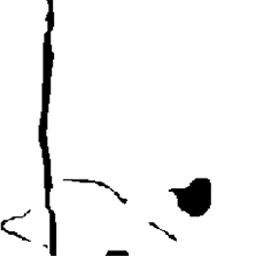
\includegraphics[width=26cm,height=25.8cm]{./images/env1.png},
};
\node[canvas is zy plane at x=0, xscale=-1, inner sep=0pt,above=\abovecaptionskip of img_output2,text width=\linewidth]
    { };

\pic[shift={(0.25,0,0)}] at (output_layer2-east) 
    {Box={
        name=output_layer3,
        caption= ,
        xlabel={{1, }},
        zlabel= ,
        fill=\ConvColor,
        height=128,
        width=0.1,
        depth=128
        }
    };

\node[canvas is zy plane at x=0] (img_output3) at (output_layer3-east) {
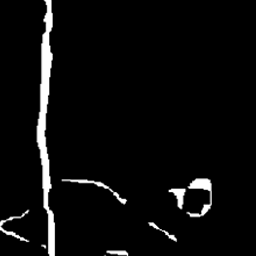
\includegraphics[width=26cm,height=25.8cm]{./images/road1.png},
};
\node[canvas is zy plane at x=0, xscale=-1, inner sep=0pt,above=\abovecaptionskip of img_output3,text width=\linewidth]
    {Output shape of segmentation mask:(256, 256, 3)};

\pic[shift={(0,0,0)}] at (10, 40, 0) 
    {Box={
        name=enc_edge_conv4,
        caption= ,
        xlabel={{1, }},
        zlabel=256,
        fill=\ConvColor,
        height=128,
        width=0.5,
        depth=128
        }
    };

\node[canvas is zy plane at x=0] (img_output_edge_enc) at (enc_edge_conv4-east) {
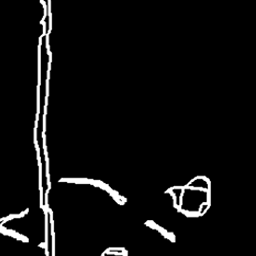
\includegraphics[width=26cm,height=25.8cm]{./images/edge1.png},
};
\node[canvas is zy plane at x=0, xscale=-1, inner sep=0pt,above=\abovecaptionskip of img_output_edge_enc,text width=\linewidth]
    {Output shape of edge encoder detector:(256, 256, 1)};

\pic[shift={ (4,0,0) }] at (enc_edge_conv4-east) 
    {Box={
        name=enc_edge_relu2,
        caption= ,
        fill=\ConvReluColor,
        opacity=0.5,
        height=128,
        width=1,
        depth=128
        }
    };

\draw [connection]  (enc_edge_relu2-west)    -- node {\midarrow} (enc_edge_conv4-east);

\pic[shift={(0,0,0)}] at (enc_edge_relu2-east) 
    {Box={
        name=enc_edge_conv2,
        caption= ,
        xlabel={{128, }},
        zlabel=256,
        fill=\ConvColor,
        height=128,
        width=4,
        depth=128
        }
    };

\pic[shift={ (0,0,0) }] at (enc_edge_conv2-east) 
    {Box={
        name=enc_edge_relu1,
        caption= ,
        fill=\ConvReluColor,
        opacity=0.5,
        height=128,
        width=1,
        depth=128
        }
    };

\pic[shift={(0,0,0)}] at (enc_edge_relu1-east) 
    {Box={
        name=enc_edge_conv1,
        caption= ,
        xlabel={{128, }},
        zlabel=256,
        fill=\ConvColor,
        height=128,
        width=4,
        depth=128
        }
    };

\pic[shift={(4,0,0)}] at (enc_edge_conv1-east) 
    {Box={
        name=enc_edge_block1_upconv1,
        caption= ,
        xlabel={{32, }},
        zlabel=256,
        fill=\AntiPoolColor,
        height=128,
        width=4,
        depth=128
        }
    };

\draw [connection]  (enc_edge_block1_upconv1-west)    -- node {\midarrow} (enc_edge_conv1-east);

\pic[shift={(4,0,0)}] at (enc_edge_block1_upconv1-east) 
    {Box={
        name=enc_edge_block2_upconv1,
        caption= ,
        xlabel={{32, }},
        zlabel=128,
        fill=\AntiPoolColor,
        height=64,
        width=4,
        depth=64
        }
    };

\draw [connection]  (enc_edge_block2_upconv1-west)    -- node {\midarrow} (enc_edge_block1_upconv1-east);

\pic[shift={(4,0,0)}] at (enc_edge_block2_upconv1-east) 
    {Box={
        name=enc_edge_block3_upconv1,
        caption= ,
        xlabel={{64, }},
        zlabel=64,
        fill=\AntiPoolColor,
        height=32,
        width=4,
        depth=32
        }
    };

\draw [connection]  (enc_edge_block3_upconv1-west)    -- node {\midarrow} (enc_edge_block2_upconv1-east);

\pic[shift={(4,0,0)}] at (enc_edge_block3_upconv1-east) 
    {Box={
        name=enc_edge_block4_upconv1,
        caption= ,
        xlabel={{64, }},
        zlabel=32,
        fill=\AntiPoolColor,
        height=16,
        width=4,
        depth=16
        }
    };

\draw [connection]  (enc_edge_block4_upconv1-west)    -- node {\midarrow} (enc_edge_block3_upconv1-east);

\pic[shift={(4,0,0)}] at (enc_edge_block4_upconv1-east) 
    {Box={
        name=enc_edge_block5_upconv1,
        caption= ,
        xlabel={{128, }},
        zlabel=16,
        fill=\AntiPoolColor,
        height=8,
        width=4,
        depth=8
        }
    };

\draw [connection]  (enc_edge_block5_upconv1-west)    -- node {\midarrow} (enc_edge_block4_upconv1-east);
\path (stage4_unit3_conv2-east) -- (block4_mxp-west) coordinate[pos=0.4] (after1);\draw [connection]  (after1)  
        -- node {\midarrow} ++(0,40,0)  
        -- node {\midarrow} ++(0,0,0)  
        -- node {\midarrow} (enc_edge_block5_upconv1-east);
        \path (stage3_unit6_conv2-east) -- (stage4_unit1_conv1-west) coordinate[pos=0.4] (after1);\path (enc_edge_block5_upconv1-east) -- (enc_edge_block4_upconv1-west) coordinate[pos=0.4] (before1);
        \draw [connection]  (after1)  
        -- node {\midarrow} ++(0,20,0)  
        -- node {\midarrow} ++(-5.35,0,0)  
        -- node {\midarrow} (before1);
        \path (stage2_unit4_conv2-east) -- (stage3_unit1_conv1-west) coordinate[pos=0.4] (after1);\path (enc_edge_block4_upconv1-east) -- (enc_edge_block3_upconv1-west) coordinate[pos=0.4] (before1);
        \draw [connection]  (after1)  
        -- node {\midarrow} ++(0,10,0)  
        -- node {\midarrow} ++(7.45,0,0)  
        -- node {\midarrow} (before1);
        \path (stage1_unit3_conv2-east) -- (stage2_unit1_conv1-west) coordinate[pos=0.4] (after1);\path (enc_edge_block3_upconv1-east) -- (enc_edge_block2_upconv1-west) coordinate[pos=0.4] (before1);
        \draw [connection]  (after1)  
        -- node {\midarrow} ++(0,15,0)  
        -- node {\midarrow} ++(15.45,0,0)  
        -- node {\midarrow} (before1);
        \path (conv0-east) -- (pooling0-west) coordinate[pos=0.4] (after1);\path (enc_edge_block1_upconv1-east) -- (enc_edge_block2_upconv1-west) coordinate[pos=0.4] (before1);
        \draw [connection]  (after1)  
        -- node {\midarrow} ++(0,20,0)  
        -- node {\midarrow} ++(21.6,0,0)  
        -- node {\midarrow} (before1);
        
\pic[shift={(2,40,0)}] at (de_block1_conv2-east) 
    {Box={
        name=dec_edge_block1_upconv1,
        caption= ,
        xlabel={{128, }},
        zlabel=16,
        fill=\AntiPoolColor,
        height=8,
        width=4,
        depth=8
        }
    };

\pic[shift={(4,0,0)}] at (dec_edge_block1_upconv1-east) 
    {Box={
        name=dec_edge_block2_upconv1,
        caption= ,
        xlabel={{64, }},
        zlabel=32,
        fill=\AntiPoolColor,
        height=16,
        width=4,
        depth=16
        }
    };

\draw [connection]  (dec_edge_block1_upconv1-west)    -- node {\midarrow} (dec_edge_block2_upconv1-east);

\pic[shift={(4,0,0)}] at (dec_edge_block2_upconv1-east) 
    {Box={
        name=dec_edge_block3_upconv1,
        caption= ,
        xlabel={{64, }},
        zlabel=64,
        fill=\AntiPoolColor,
        height=32,
        width=4,
        depth=32
        }
    };

\draw [connection]  (dec_edge_block2_upconv1-west)    -- node {\midarrow} (dec_edge_block3_upconv1-east);

\pic[shift={(4,0,0)}] at (dec_edge_block3_upconv1-east) 
    {Box={
        name=dec_edge_block4_upconv1,
        caption= ,
        xlabel={{32, }},
        zlabel=128,
        fill=\AntiPoolColor,
        height=64,
        width=4,
        depth=64
        }
    };

\draw [connection]  (dec_edge_block3_upconv1-west)    -- node {\midarrow} (dec_edge_block4_upconv1-east);

\pic[shift={(4,0,0)}] at (dec_edge_block4_upconv1-east) 
    {Box={
        name=dec_edge_block5_upconv1,
        caption= ,
        xlabel={{32, }},
        zlabel=256,
        fill=\AntiPoolColor,
        height=128,
        width=4,
        depth=128
        }
    };

\draw [connection]  (dec_edge_block4_upconv1-west)    -- node {\midarrow} (dec_edge_block5_upconv1-east);

\pic[shift={(4,0,0)}] at (dec_edge_block5_upconv1-east) 
    {Box={
        name=dec_edge_conv1,
        caption= ,
        xlabel={{128, }},
        zlabel=256,
        fill=\ConvColor,
        height=128,
        width=4,
        depth=128
        }
    };

\draw [connection]  (dec_edge_block5_upconv1-west)    -- node {\midarrow} (dec_edge_conv1-east);

\pic[shift={ (0,0,0) }] at (dec_edge_conv1-east) 
    {Box={
        name=dec_edge_relu1,
        caption= ,
        fill=\ConvReluColor,
        opacity=0.5,
        height=128,
        width=1,
        depth=128
        }
    };

\pic[shift={(0,0,0)}] at (dec_edge_relu1-east) 
    {Box={
        name=dec_edge_conv2,
        caption= ,
        xlabel={{128, }},
        zlabel=256,
        fill=\ConvColor,
        height=128,
        width=4,
        depth=128
        }
    };

\pic[shift={ (0,0,0) }] at (dec_edge_conv2-east) 
    {Box={
        name=dec_edge_relu2,
        caption= ,
        fill=\ConvReluColor,
        opacity=0.5,
        height=128,
        width=1,
        depth=128
        }
    };

\pic[shift={(4,0,0)}] at (dec_edge_relu2-east) 
    {Box={
        name=dec_edge_conv4,
        caption= ,
        xlabel={{1, }},
        zlabel=256,
        fill=\ConvColor,
        height=128,
        width=0.5,
        depth=128
        }
    };

\node[canvas is zy plane at x=0] (img_output_edge_enc) at (dec_edge_conv4-east) {
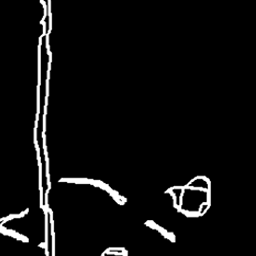
\includegraphics[width=26cm,height=25.8cm]{./images/edge1.png},
};
\node[canvas is zy plane at x=0, xscale=-1, inner sep=0pt,above=\abovecaptionskip of img_output_edge_enc,text width=\linewidth]
    {Output shape of edge decoder detector:(256, 256, 1)};

\draw [connection]  (dec_edge_relu2-west)    -- node {\midarrow} (dec_edge_conv4-east);
\path (de_block1_conv2-east) -- (de_block1_upconv1-west) coordinate[pos=0.4] (after1);\draw [connection]  (after1)  
        -- node {\midarrow} ++(0,40,0)  
        -- node {\midarrow} ++(0,0,0)  
        -- node {\midarrow} (dec_edge_block1_upconv1-east);
        \path (de_block2_conv2-east) -- (de_block2_upconv1-west) coordinate[pos=0.4] (after1);\path (dec_edge_block1_upconv1-east) -- (dec_edge_block2_upconv1-west) coordinate[pos=0.4] (before1);
        \draw [connection]  (after1)  
        -- node {\midarrow} ++(0,5,0)  
        -- node {\midarrow} ++(-1.9,0,0)  
        -- node {\midarrow} (before1);
        \path (de_block3_conv2-east) -- (de_block3_upconv1-west) coordinate[pos=0.4] (after1);\path (dec_edge_block2_upconv1-east) -- (dec_edge_block3_upconv1-west) coordinate[pos=0.4] (before1);
        \draw [connection]  (after1)  
        -- node {\midarrow} ++(0,10,0)  
        -- node {\midarrow} ++(-2.9,0,0)  
        -- node {\midarrow} (before1);
        \path (de_block4_conv2-east) -- (de_block4_upconv1-west) coordinate[pos=0.4] (after1);\path (dec_edge_block3_upconv1-east) -- (dec_edge_block4_upconv1-west) coordinate[pos=0.4] (before1);
        \draw [connection]  (after1)  
        -- node {\midarrow} ++(0,15,0)  
        -- node {\midarrow} ++(-3.9,0,0)  
        -- node {\midarrow} (before1);
        \path (de_block5_conv2-east) -- (de_block5_upconv1-west) coordinate[pos=0.4] (after1);\path (dec_edge_block4_upconv1-east) -- (dec_edge_block5_upconv1-west) coordinate[pos=0.4] (before1);
        \draw [connection]  (after1)  
        -- node {\midarrow} ++(0,17.5,0)  
        -- node {\midarrow} ++(-4.9,0,0)  
        -- node {\midarrow} (before1);
        \path (de_block6_conv2-east) -- (de_block7_conv1-west) coordinate[pos=0.4] (after1);\path (dec_edge_block5_upconv1-east) -- (dec_edge_conv1-west) coordinate[pos=0.4] (before1);
        \draw [connection]  (after1)  
        -- node {\midarrow} ++(0,20,0)  
        -- node {\midarrow} ++(-5.9,0,0)  
        -- node {\midarrow} (before1);
        
\node[above,font=\fontsize{70pt}{70pt}\bfseries,] at (current bounding box.north) {U-NET + ERN by Alexander D. Rios};
\end{tikzpicture}
\end{document}
